% Created 2018-03-05 Mon 22:22
% Intended LaTeX compiler: pdflatex
\documentclass[11pt]{article}
\usepackage[utf8]{inputenc}
\usepackage[T1]{fontenc}
\usepackage{graphicx}
\usepackage{grffile}
\usepackage{longtable}
\usepackage{wrapfig}
\usepackage{rotating}
\usepackage[normalem]{ulem}
\usepackage{amsmath}
\usepackage{textcomp}
\usepackage{amssymb}
\usepackage{capt-of}
\usepackage{hyperref}
\author{Petr Blaho, Ilya Etingof}
\date{\today}
\title{PA200 - Cloud Computing Concepts}
\hypersetup{
 pdfauthor={Petr Blaho, Ilya Etingof},
 pdftitle={PA200 - Cloud Computing Concepts},
 pdfkeywords={},
 pdfsubject={},
 pdfcreator={Emacs 25.3.1 (Org mode 9.1.7)}, 
 pdflang={English}}
\begin{document}

\maketitle


\section*{Virtualization}
\label{sec:org94f2f02}

\section*{Warm-up}
\label{sec:org14080cd}
\begin{itemize}
\item What is cloud computing?
\item Cloud traits?
\item Cloud deployment models?
\end{itemize}

\section*{What is cloud computing?}
\label{sec:orge3bf509}
\begin{enumerate}
\item Usage model of computer resources
\item Networked computers
\item Distributed computing technology
\item A collection of heterogeneous computers
\end{enumerate}

\section*{Cloud traits?}
\label{sec:org78ee609}
\begin{enumerate}
\item High availability
\item On-demand self-service
\item High performance
\item Broad network access
\item Resource pooling
\item Rapid elasticity
\item Measured Service
\end{enumerate}

\section*{Cloud service models?}
\label{sec:orga335e97}
\begin{enumerate}
\item Software as a Service
\item Application as a Service
\item Platform as a Service
\item Infrastructure as a Service
\item Data as a Service
\end{enumerate}

\section*{Cloud deployment models}
\label{sec:orgda66f46}
\begin{enumerate}
\item Public Cloud
\item Private Cloud
\item Hybrid Cloud
\item Personal Cloud
\item Community Cloud
\item Enterprise Cloud
\end{enumerate}

\section*{History of virtualization}
\label{sec:orgf92238a}
\begin{itemize}
\item How old is virtualization?
\end{itemize}

\section*{History of virtualization}
\label{sec:org8ad1d5e}
\begin{itemize}
\item Early 1960: batch processing
\item 1967: first time-sharing system - IBM S/370-67
\item 2005: Intel VT-x, AMD-V - new instruction set
\item 2005-: VMware, VirtualBox, KVM\ldots{}
\end{itemize}

\section*{What exactly is virtualization?}
\label{sec:org8cf695f}
\begin{itemize}
\item Multi-programming vs multi-tasking
\item Multi-threading vs multi-tasking vs virtualization?
\item Containers vs OS virtualization
\item CPUs: Multi-core vs Hyper-threading
\end{itemize}

\section*{How did virtualization work before 2005?}
\label{sec:orgf8e6a59}
\begin{itemize}
\item Well, sloooowly\ldots{}
\item Basing on 80386 CPU features
\end{itemize}

\section*{Is it cloud already?}
\label{sec:org25e29ea}
\begin{itemize}
\item What is virtualization?
\item What is cloud?
\end{itemize}

\section*{Is it cloud already?}
\label{sec:org3dce481}
\begin{itemize}
\item Hypervisors
\item Virtualization management and services
\end{itemize}

\section*{Hypervisors}
\label{sec:orgb42cbe7}
\begin{itemize}
\item Native or bare-metal
\item Hosted
\end{itemize}

\subsection*{Hypervisors}
\label{sec:org21c2943}
\begin{center}
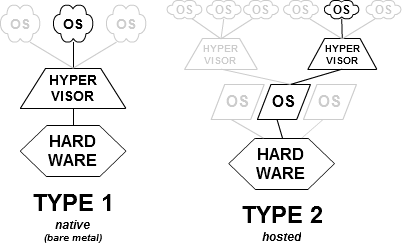
\includegraphics[width=.9\linewidth]{./hyperviseur.png}
\end{center}

\section*{Full or para-virtualization}
\label{sec:org054d3ae}
\begin{itemize}
\item Full: unmodified OS on top of hypervisor
\item Para: modified OS calls hypervisor API
\end{itemize}

\section*{Examples of native hypervisors}
\label{sec:org9a22dc6}
\begin{itemize}
\item XEN
\item MS Hyper-V
\item VMware ESXi
\end{itemize}

\section*{Examples of hosted hypervisors}
\label{sec:orgb1e497f}
\begin{itemize}
\item QEMU
\item KVM
\item VirtualBox
\item VMware Workstation
\item FreeBSD bhyve
\end{itemize}

\section*{XEN}
\label{sec:org1a97271}
\begin{itemize}
\item founded in 2003 by XenSource, bought in 2007 by Citrix
\item 2013 under Linux Foundation as Xen Project
\item native hypervisor
\end{itemize}

\section*{ZEN}
\label{sec:org9b5c7e6}
\begin{center}
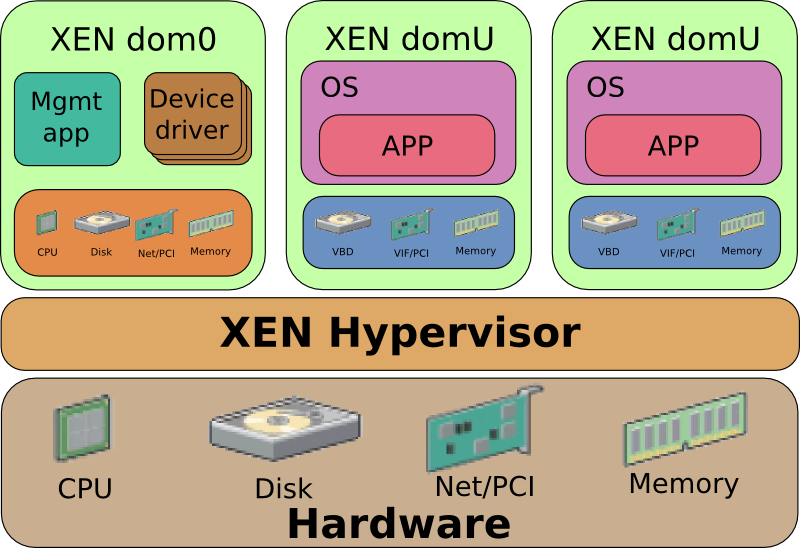
\includegraphics[width=.9\linewidth]{./xen.png}
\end{center}

\section*{KVM}
\label{sec:orgd4b4dc4}
\begin{itemize}
\item Modular kernel virtualization
\item provides user space access to hw virtualization
\item started by Qumranet
\item 2007 merged into linux kernel
\end{itemize}

\section*{KVM}
\label{sec:orgc2437dd}
\begin{center}
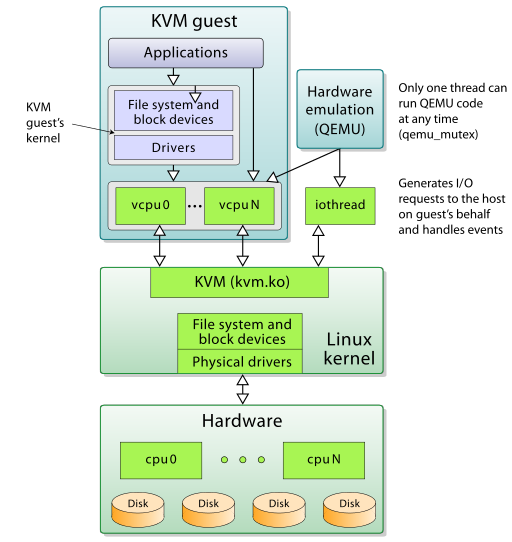
\includegraphics[width=.9\linewidth]{./kvm.png}
\end{center}

\section*{QEMU}
\label{sec:org3db92ce}
\begin{itemize}
\item hosted hypervisor
\item provides CPU and/or hardware emulation
\item can be used with KVM (hardware-only emulation)
\end{itemize}

\section*{QEMU}
\label{sec:org99a0717}
\begin{itemize}
\item Other practical QEMU use-cases?
\end{itemize}

\section*{Type 1 vs type 2 confusion}
\label{sec:orged94567}
\begin{itemize}
\item Linux with KVM
\item FreeBSD with bhyve
\end{itemize}

\section*{Full vs para-virtualization}
\label{sec:org1f63315}
\begin{itemize}
\item Full: run unmodified OS image
\item Para: OS explicitly calls hypervisor
\end{itemize}

\section*{Para-virtualization}
\label{sec:org15fae2b}
\begin{itemize}
\item Why?
\end{itemize}

\subsection*{Why is it called Hypervisor?}
\label{sec:org8369eb8}
\begin{itemize}
\item What's behind the name?
\end{itemize}

\section*{Virtualization management}
\label{sec:org5e1f11d}
\begin{itemize}
\item Common API to different hypervisors
\item High-level VM lifecycle abstraction
\item Cloud services: networks, storage\ldots{}
\end{itemize}

\section*{Cloud services}
\label{sec:orgb6ae2d0}
\begin{itemize}
\item OS image deployment
\item Centralized OS configuration
\item Automated network configuration
\item Instance backup/snapshot/migration
\item Centralized user authentication
\item Centralized storage
\item User interface
\end{itemize}

\section*{Examples of virtualization software}
\label{sec:org96d9213}
\begin{itemize}
\item libvirt
\item oVirt
\item OpenStack
\end{itemize}

\section*{Libvirt}
\label{sec:orgc8d5c5f}
\begin{itemize}
\item Common API for hypervisor type abstraction supports
\item LXC
\item KVM/QEMU, Xen, VirtualBox
\item VMware ESXi and Workstation
\item MS Hyper-V, IBM PowerVM
\end{itemize}

\section*{Libvirt}
\label{sec:orge686a84}
\begin{center}
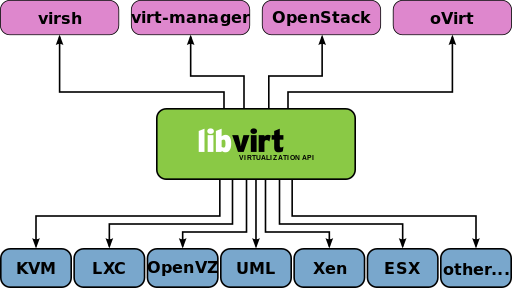
\includegraphics[width=.9\linewidth]{./libvirt.png}
\end{center}

\section*{oVirt}
\label{sec:org9e02eca}
\begin{itemize}
\item Virtualization management platform
\item On top of KVM
\item Upstream for RHV
\item Engine
\item Node
\item VDSM - virtual desktop and server manager
\end{itemize}

\section*{OpenStack}
\label{sec:org4808092}
\begin{itemize}
\item Software platform for cloud computing
\item Started in 2010 by Rackspace and NASA
\item In 2012 founded OpenStack Foundation
\end{itemize}

\section*{OpenStack}
\label{sec:orgad024a2}
\begin{center}
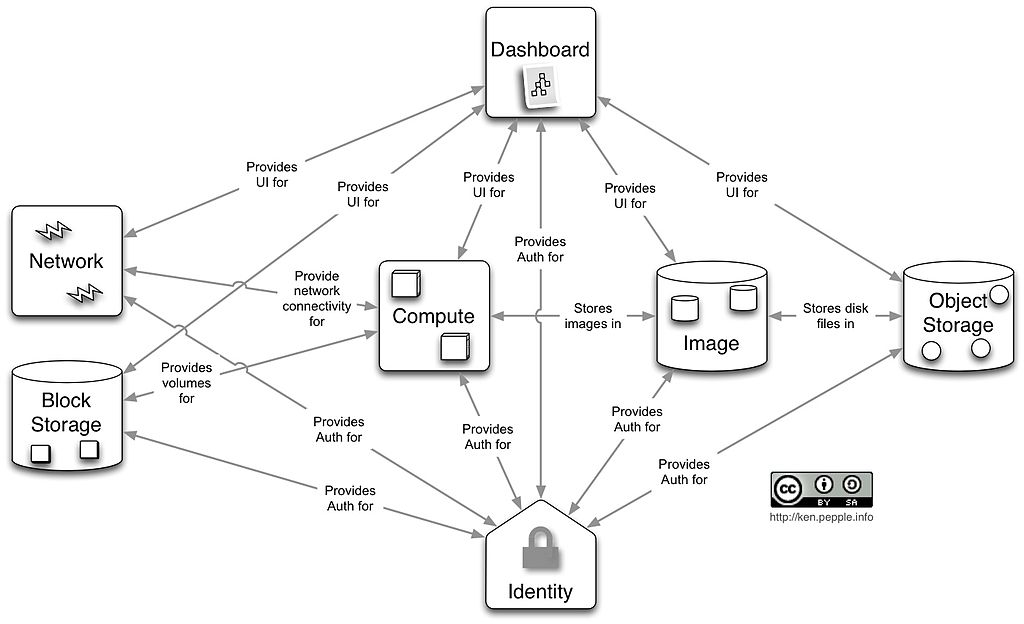
\includegraphics[width=.9\linewidth]{./openstack.jpg}
\end{center}

\section*{OpenStack}
\label{sec:org6683d3e}
\begin{center}
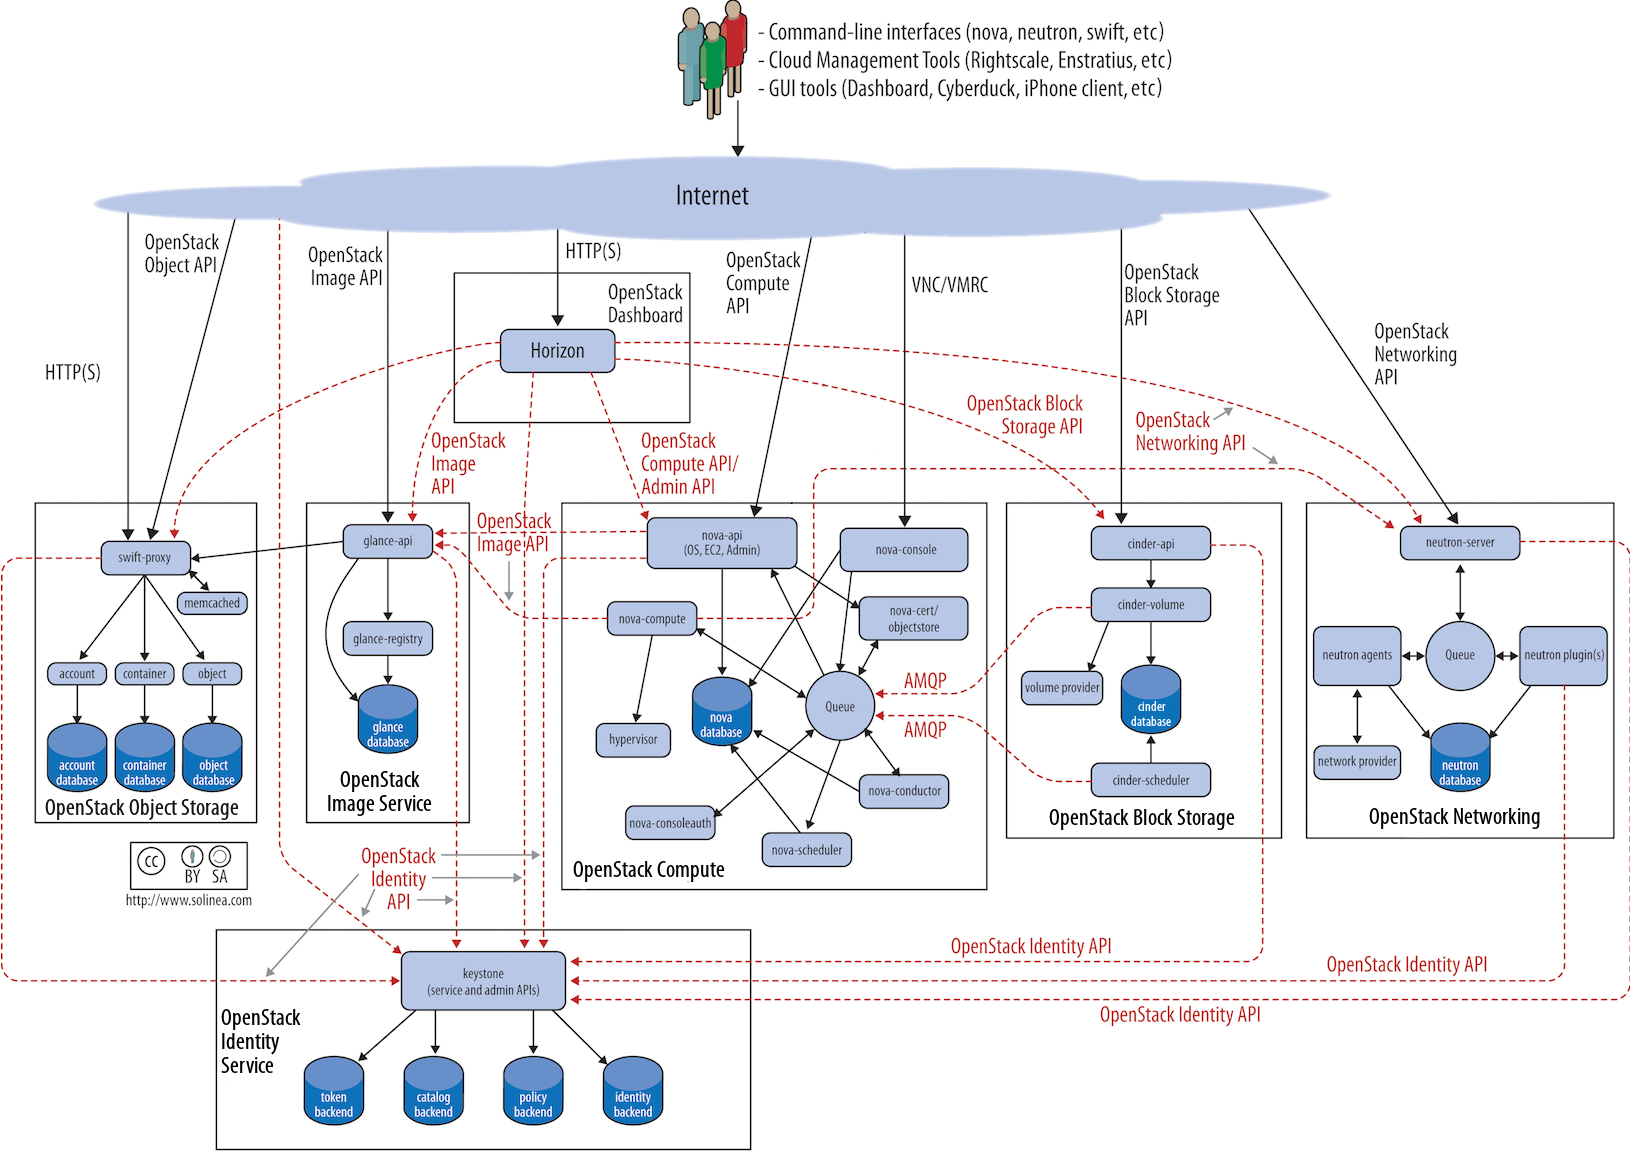
\includegraphics[width=.9\linewidth]{./openstack-detailed.png}
\end{center}

\section*{Hypervisors vs Containers}
\label{sec:org8944238}
\begin{itemize}
\item Hypervisors spawn VMs
\item Containers isolates apps to namespaces
\end{itemize}

\section*{Example container software}
\label{sec:org82eef8c}
\begin{itemize}
\item Docker
\item LXC
\item OpenVZ
\item chroot
\end{itemize}

\section*{Cloud features}
\label{sec:org047efe8}
\begin{itemize}
\item Easy provisioning and configuration
\item Movable resource: snapshot/backup/live migration
\item Consolidation of resources: scale up/down
\end{itemize}

\subsection*{Cloud features}
\label{sec:org6784578}
\begin{itemize}
\item Isolation from host HW and OS
\item Virtual vs Physical machine monitoring
\item Easier testing and evaluation
\item Duplication of environments
\end{itemize}

\section*{Recap: the age of virtualization?}
\label{sec:org53f6e3f}
\begin{enumerate}
\item IBM 700/7000, since 1952
\item CP-40 research project, early sixties
\item IBM S/370-67, 1966
\item Gameframes, since 2007
\item Intel VT-x, AMD-V, since 2005
\end{enumerate}

\section*{Recap: virtualization technologies?}
\label{sec:orgd8e064c}
\begin{enumerate}
\item Multi-tasking
\item Multi-threading processes
\item Containers
\item Hyper-threading CPU
\item Multi-core CPU
\item Intel VT-x, AMD-V
\item Multi-programming
\end{enumerate}

\section*{Recap: hypervisor types?}
\label{sec:org2d754bf}
\begin{enumerate}
\item Hybryd
\item Bare-metal
\item Native
\item Hosted
\item Para-hypervisor
\end{enumerate}

\section*{Recap: what makes up a cloud?}
\label{sec:org359c1ab}
\begin{enumerate}
\item One hypervisor
\item One or more hypervisors
\item Baremetal computers
\item Baremetal switches and routers
\item Networking service
\end{enumerate}

\section*{Recap: virtualization vs containers?}
\label{sec:orga852fc0}
\begin{enumerate}
\item We can run OS in a container
\item We can run different OS'es in containers
\item We can run VM in a container
\item Containers are more secure than VM
\item Containers consume less resources than VM
\item We can run Windows app in Linux container
\end{enumerate}

\section*{Bonus question: matreshka cloud?}
\label{sec:org356476b}
\begin{itemize}
\item Can you run a cloud in a cloud?
\end{itemize}
\end{document}